\documentclass{beamer}
\usepackage[T1]{fontenc}
\usepackage[utf8]{inputenc}
\usepackage[italian]{babel}
\usepackage{upgreek}
\usepackage{epstopdf}
\usepackage{tikz}

\title[Simulazione Ising 2D]
{Simulazione di un reticolo di \\ Ising bidimensionale in CUDA}
\author{Stefano Mandelli}
\date{14 Luglio 2016}
\usetheme{Warsaw}
\setbeamertemplate{navigation symbols}{}

\begin{document}

%FRAME 1

	\begin{frame}
 		\maketitle
	\end{frame}
 
%-----------------Ricevitore RF---------------% 

%FRAME 2

	\begin{frame}
		\frametitle{Il Modello di Ising}
		Il modello di Ising \`e caratterizzato dalla seguente Hamiltoniana
		\begin{eqnarray}
			H = -J \sum_{\left\langle i,j \right\rangle} s_i s_j -h\sum_i s_i
		\end{eqnarray}
		le cui grandezze fisiche di interesse sono la magnetizzazione media e il calore specifico per spin definiti come
		\begin{eqnarray}
			m=\frac{1}{N}\left\langle \sum_i s_i\right\rangle \,\,,\,\, c_v = \frac{\beta^2 k_B^2}{N} \left(\left\langle E\right\rangle^2 - \left\langle E^2\right\rangle \right)
		\end{eqnarray}
	\end{frame}

	\begin{frame}
		\frametitle{Algoritmo di Metropolis}
		L'algoritmo con cui vengono proposti gli update degli spin \`e quello di metropolis la cui probabilit\`a di accettazione \`e data da
		\begin{figure}
			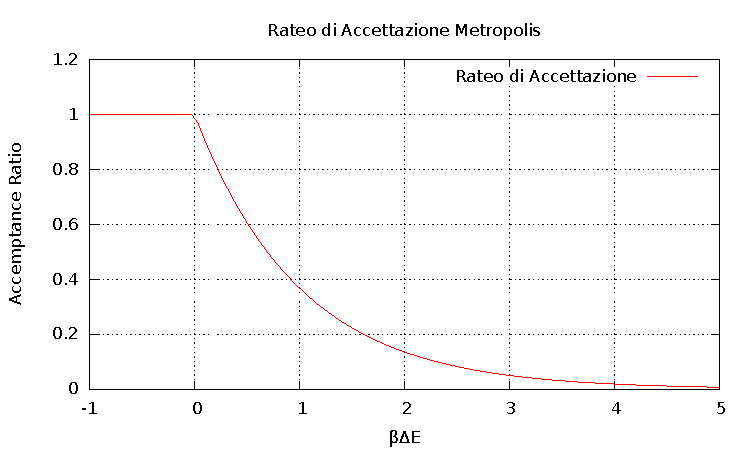
\includegraphics[scale=0.85]{../acc_rat.pdf}
		\end{figure}
	\end{frame}

	
	\begin{frame}
		\frametitle{Implementazione del codice su GPU}
		Ottimizzazione su memoria shared del reticolo attraverso aggiornamento su doppia scacchiera
		\begin{figure}
	\begin{center}
		\begin{tikzpicture}[x=0.8cm,y=0.8cm]
		
		\foreach \p in {0,1,...,6}{
				\draw [ultra thick] (\p,0) -- (\p,6);
				\draw [ultra thick] (0,\p) -- (6,\p);
			}
		\foreach \p in {0,0.5,...,18}{
				\draw (\p/3,0) -- (\p/3,6);
				\draw (0,\p/3) -- (6,\p/3);
			}

		\foreach \blockx in {0,2,...,5}{
				\foreach \blocky in {0,2,...,5}{
					\fill [fill=red, opacity=0.5] (\blockx,\blocky) rectangle (\blockx+1,\blocky+1);
			}
		}
		\foreach \blockx in {0,2,...,5}{
				\foreach \blocky in {0,2,...,5}{
					\fill [fill=red, opacity=0.5] (\blockx+1,\blocky+1) rectangle (\blockx+2,\blocky+2);
			}
		}

		\fill [fill=yellow, opacity=0.7] (1,2) rectangle (2,2+0.5/3);
		\fill [fill=yellow, opacity=0.7] (1,1) rectangle (1-0.5/3,2);
		\fill [fill=yellow, opacity=0.7] (1,1) rectangle (2,1-0.5/3);
		\fill [fill=yellow, opacity=0.7] (2,1) rectangle (2+0.5/3,2);

		\foreach \a in {0,2,...,5}{
				\foreach \b in {0,2,...,5}{
					\fill [fill=black, opacity=0.7] (1+\a*0.5/3,1+\b*0.5/3) rectangle (1+\a*0.5/3+0.5/3,1+\b*0.5/3+0.5/3);
			}
	}
		\foreach \a in {0,2,...,5}{
				\foreach \b in {0,2,...,5}{
					\fill [fill=black, opacity=0.7] (1+\a*0.5/3+0.5/3,1+\b*0.5/3+0.5/3) rectangle (1+\a*0.5/3+2*0.5/3,1+\b*0.5/3+2*0.5/3);
			}
	}

		\end{tikzpicture}
	\end{center}
	\caption{Le zone rosse pi\`u le aree gialle rappresentano i blocchi di memoria \emph{shared}. Ogni blocco viene aggiornato a scacchiera. Le condizioni di raccordo blocco-blocco sono identificate dai siti reticolari colorati in giallo}
	\label{reticolo_shared}
\end{figure}


	\end{frame}


	\begin{frame}
		\frametitle{Confronto Modello Fisico}
		Confronto CPU - GPU dei grafici di magnetizzazione e calore specifico con la soluzione di Onsager al limite termodinamico
		\begin{figure}
				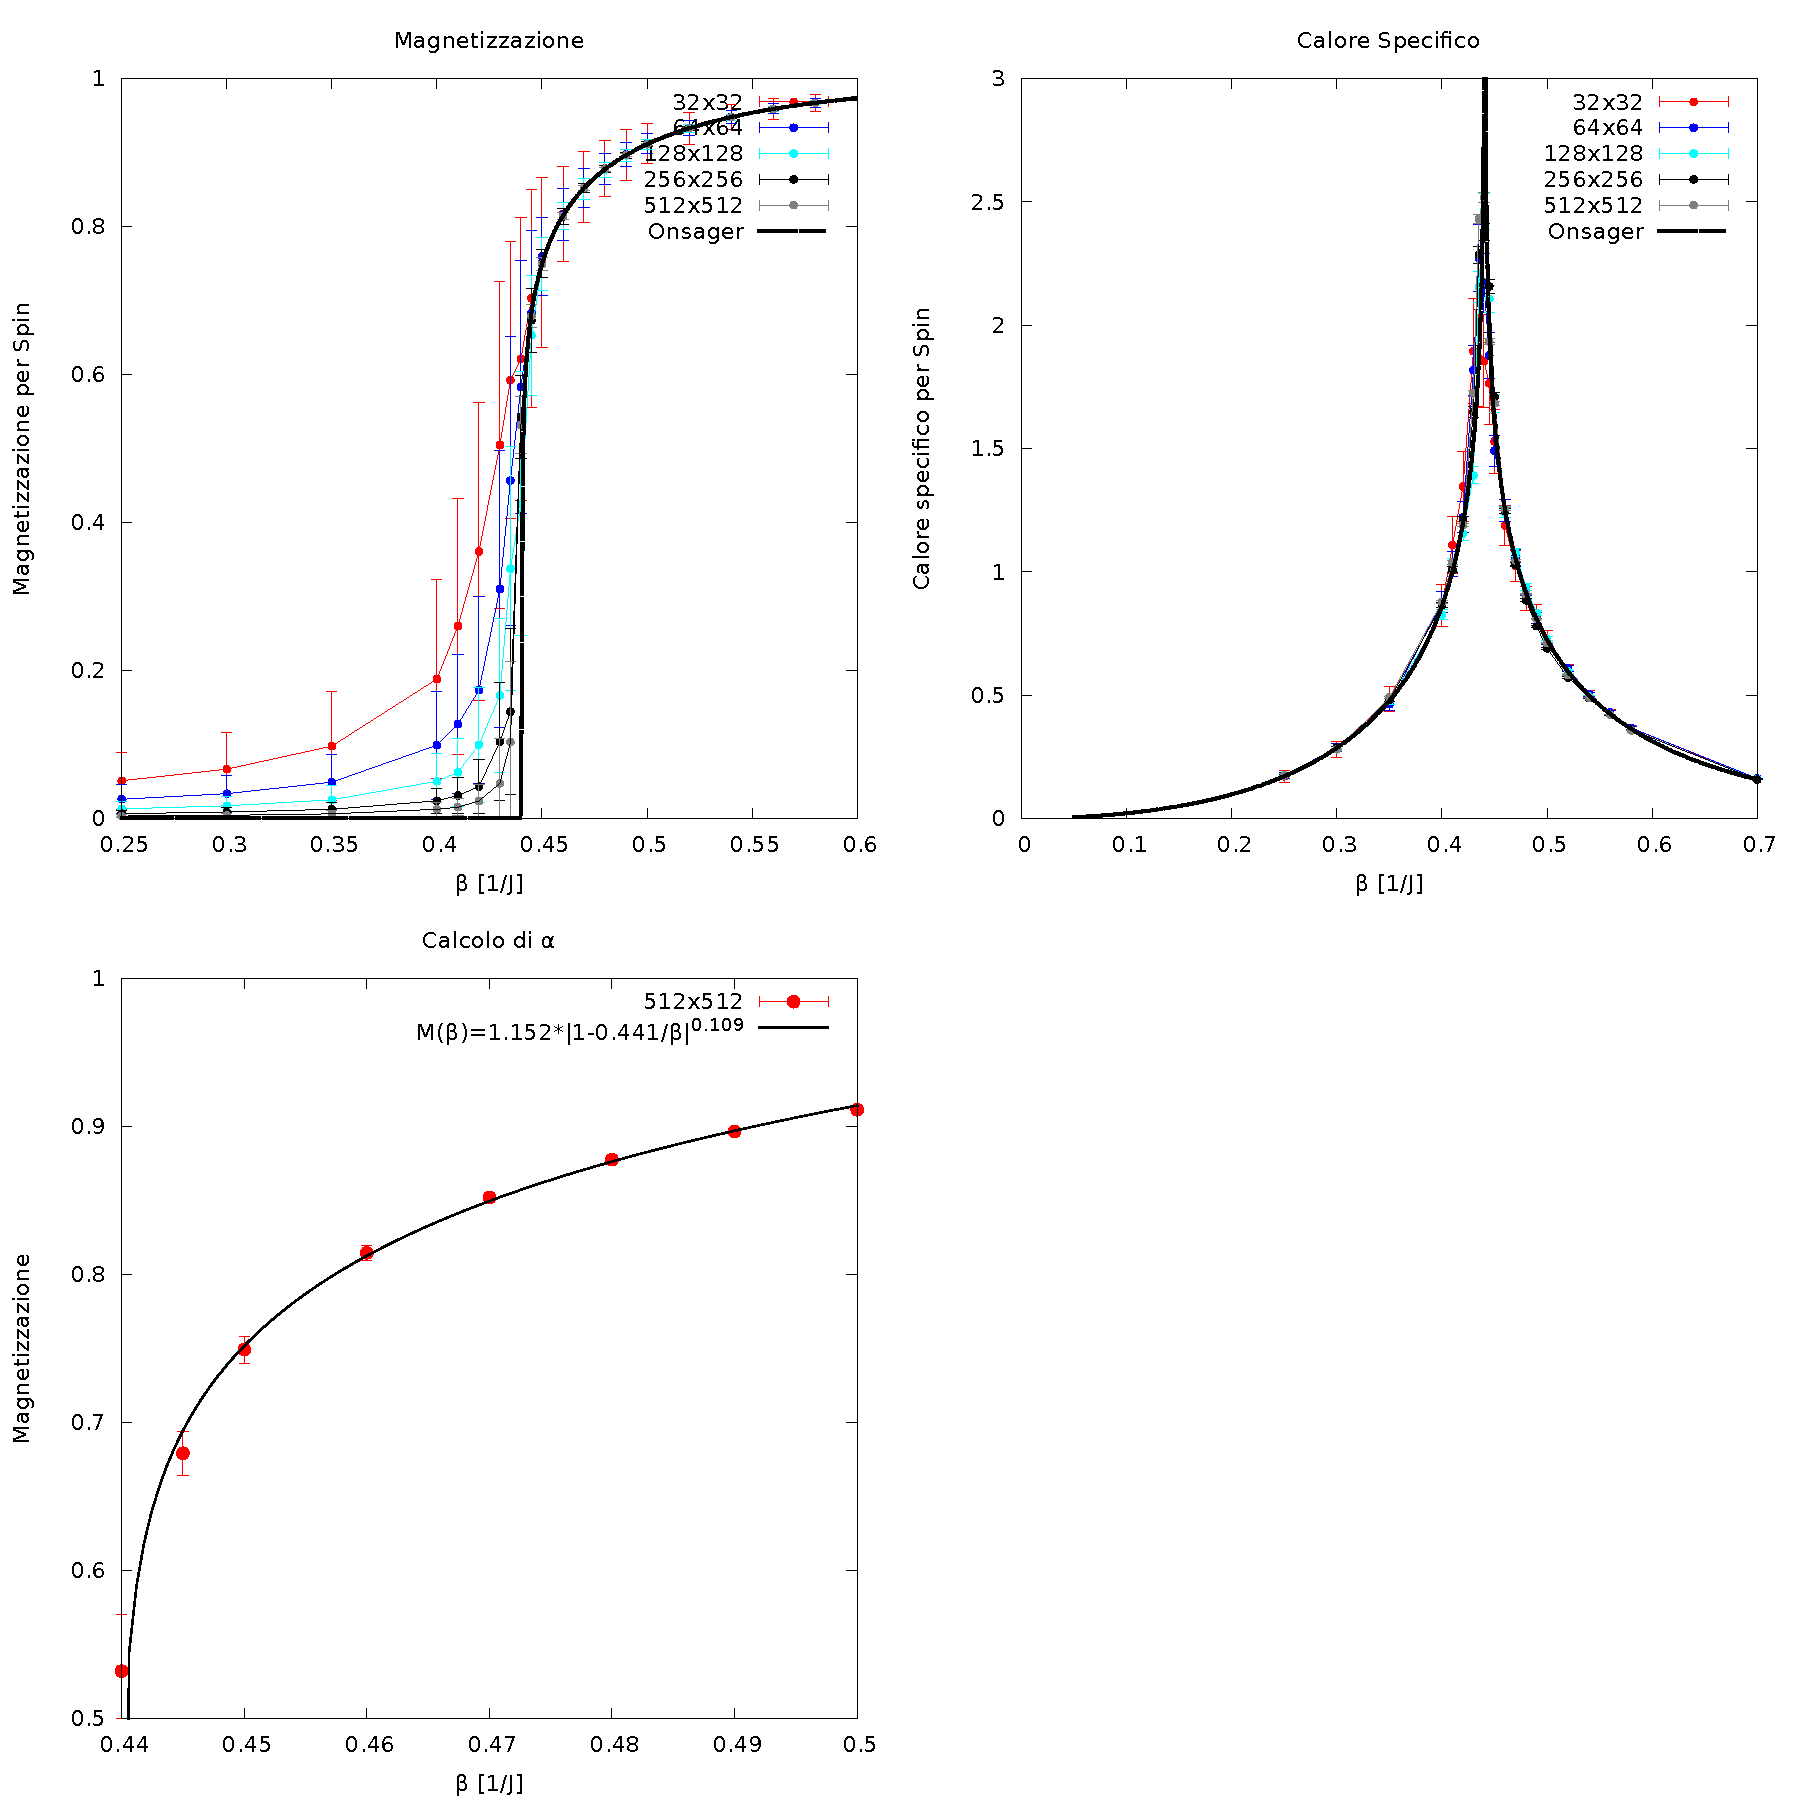
\includegraphics[scale=0.18]{../../CPU/Result/Ising_Mag_Cv.pdf}	
				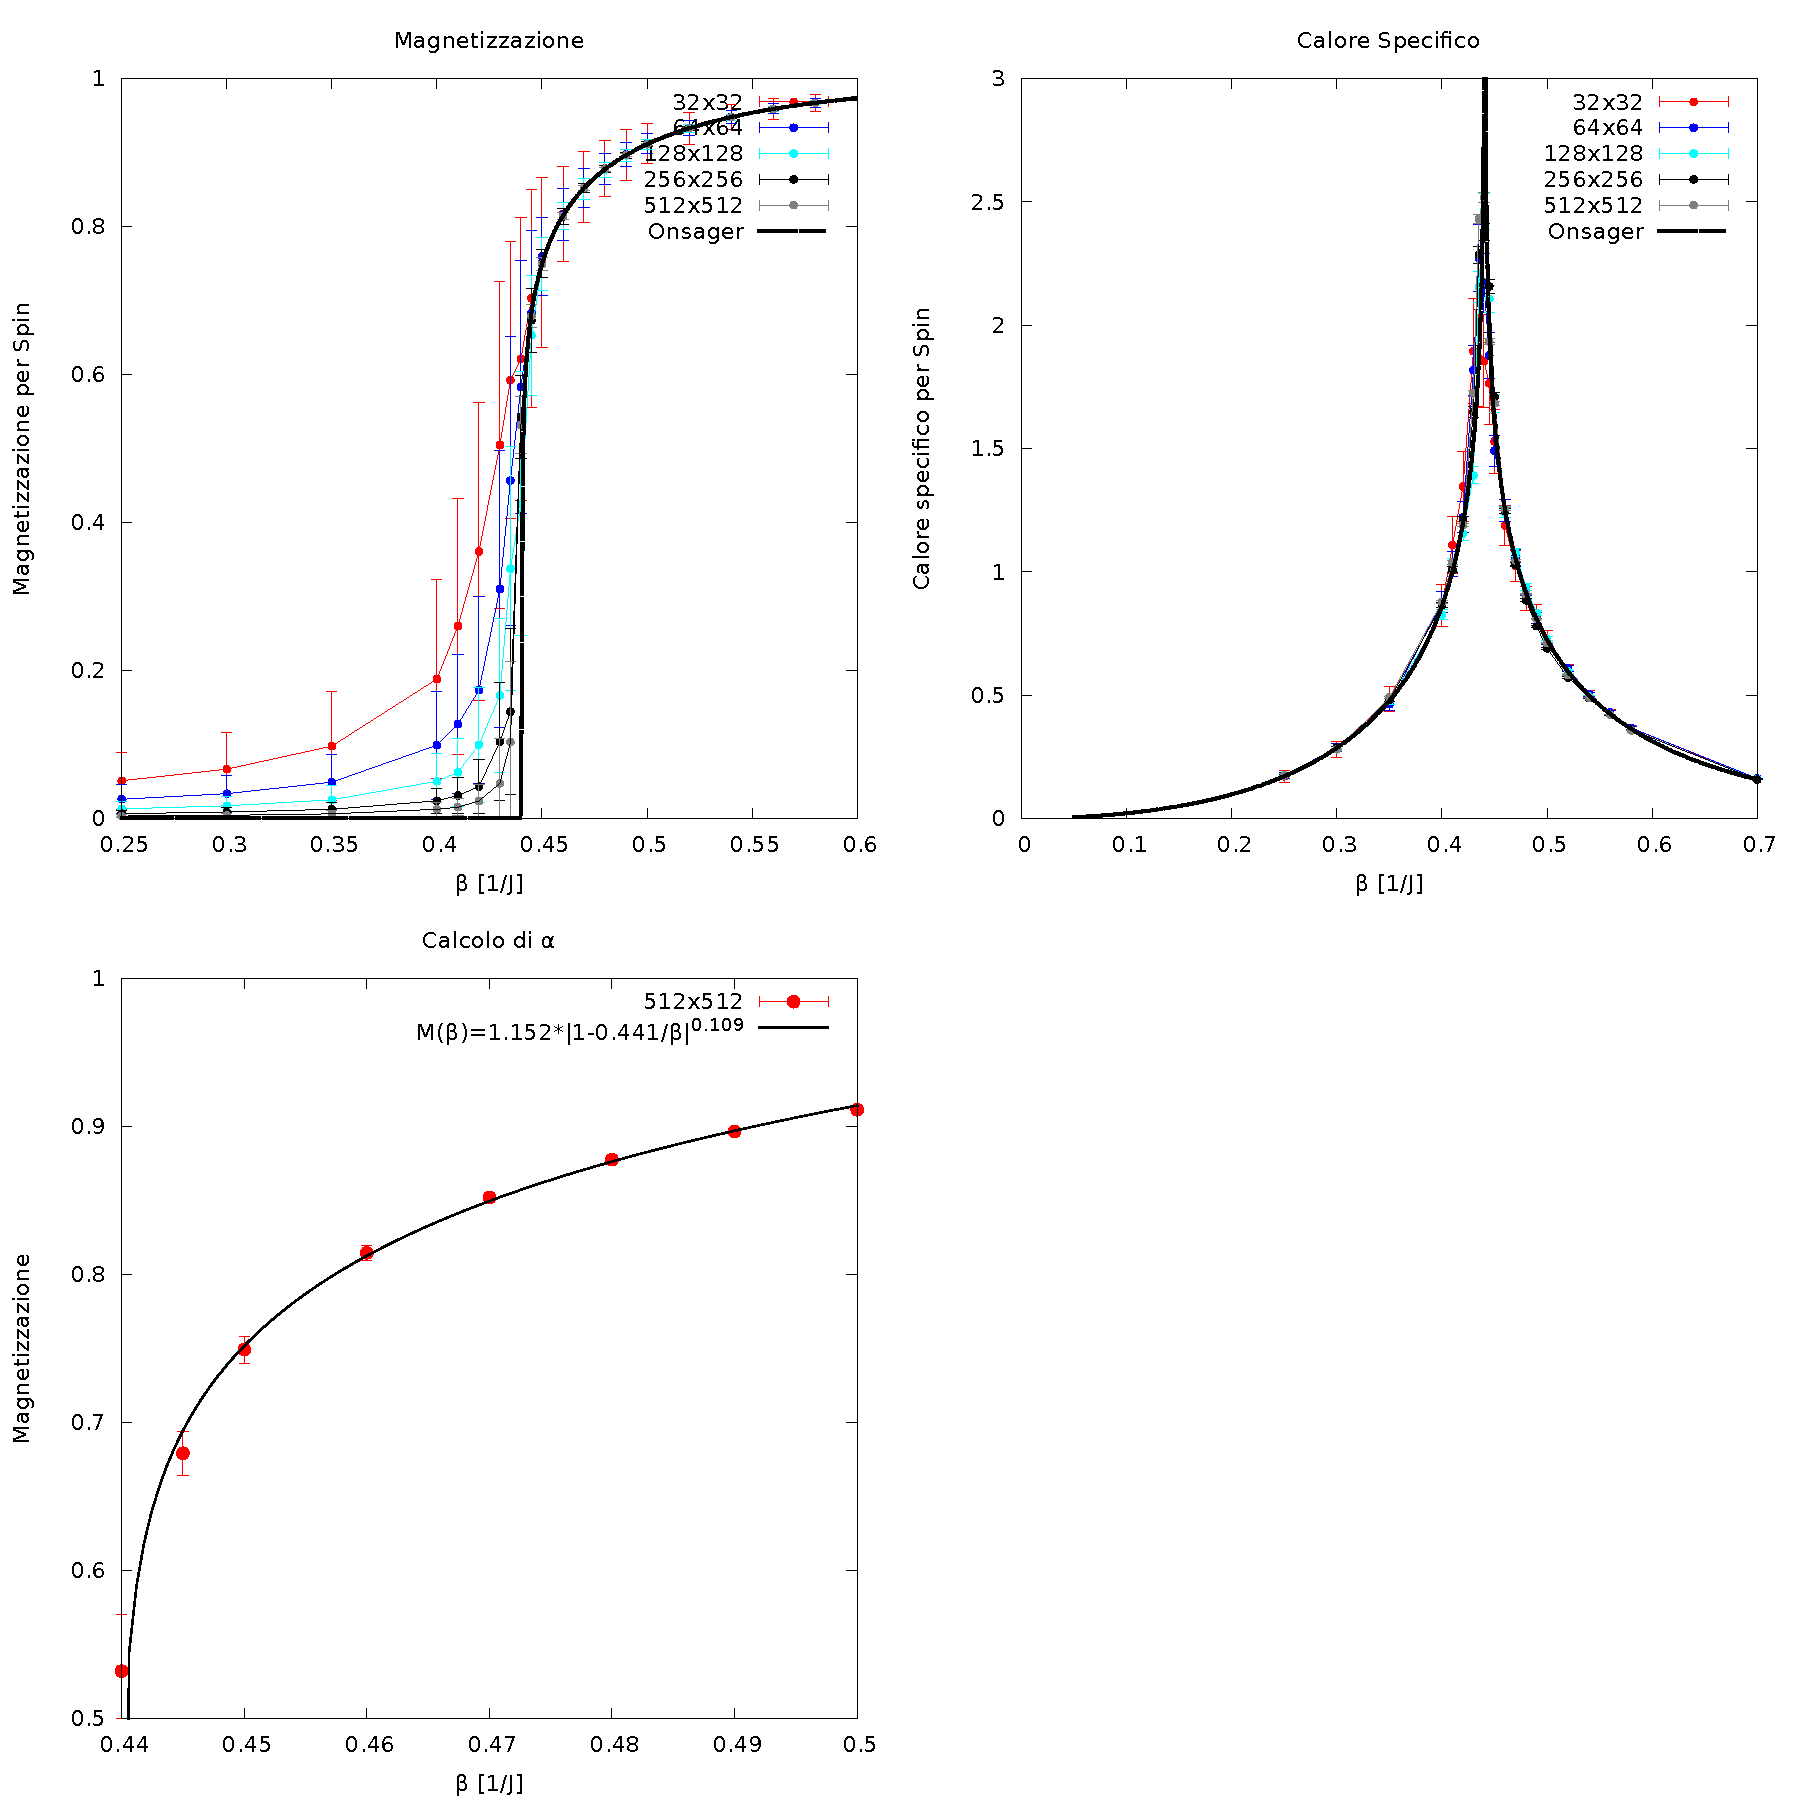
\includegraphics[scale=0.18]{../../CPU/Result/Ising_Mag_Cv.pdf}
		\end{figure}

	\end{frame}

	\begin{frame}
		\frametitle{}
	\end{frame}


\end{document}
